\PassOptionsToPackage{unicode}{hyperref}
\documentclass[aspectratio=169, professionalfonts, 9pt, bibliography=totoc, xcolor={svgnames},
hyperref={colorlinks,citecolor=tudark,linkcolor=blue,urlcolor=DarkBlue}
]{beamer}

\usefonttheme[onlymath]{serif}
\usetheme[showtotalframes]{tudo}

\usepackage{polyglossia}
\setmainlanguage{german}
\usepackage[backend=biber]{biblatex}
\addbibresource{lit.bib}

% Mathematik
\usepackage{amsmath}
\usepackage{amssymb}
\usepackage{mathtools}
\usepackage{cancel}

\usepackage{hyperref}
\usepackage{bookmark}

\mode<presentation>

\usefonttheme{professionalfonts}
\usepackage{fontspec}
\usepackage[
    math-style=ISO,
    bold-style=ISO,
    nabla=upright,
    partial=upright,
    sans-style=italic,
]{unicode-math}
\setmathfont{Latin Modern Math}
\usepackage{listings}

% Paket float verbessern
\usepackage{scrhack}

% unverzichtbare Mathe-Befehle
\usepackage{amsmath}
% viele Mathe-Symbole
\usepackage{amssymb}
% Erweiterungen für amsmath
\usepackage{mathtools}

% Fonteinstellungen
\usepackage{fontspec}

% deutsche Spracheinstellungen
\usepackage{polyglossia}
\setmainlanguage{german}

% traditionelle Fonts für Mathematik
\setmathfont{Latin Modern Math}

\setmathfont{XITS Math}[range={scr, bfscr}]
\setmathfont{XITS Math}[range={cal, bfcal}, StylisticSet=1]

% Zahlen und Einheiten
\usepackage[
  locale=DE,                   % deutsche Einstellungen
  separate-uncertainty=true,   % immer Fehler mit \pm
  per-mode=symbol-or-fraction, % / in inline math, fraction in display math
]{siunitx}

% chemische Formeln
\usepackage[
  version=4,
  math-greek=default, % ┐ mit unicode-math zusammenarbeiten
  text-greek=default, % ┘
]{mhchem}

% richtige Anführungszeichen
\usepackage[autostyle]{csquotes}

% schöne Brüche im Text
\usepackage{xfrac}

% Standardplatzierung für Floats einstellen
\usepackage{float}
\floatplacement{figure}{htbp}
\floatplacement{table}{htbp}

% Floats innerhalb einer Section halten
\usepackage[
  section, % Floats innerhalb der Section halten
  below,   % unterhalb der Section aber auf der selben Seite ist ok
]{placeins}

% Seite drehen für breite Tabellen: landscape Umgebung
\usepackage{pdflscape}

% Captions schöner machen.
\usepackage[
  labelfont=bf,        % Tabelle x: Abbildung y: ist jetzt fett
  font=small,          % Schrift etwas kleiner als Dokument
  width=0.9\textwidth, % maximale Breite einer Caption schmaler
]{caption}
% subfigure, subtable, subref
\usepackage{subcaption}

% Grafiken können eingebunden werden
\usepackage{graphicx}
% größere Variation von Dateinamen möglich
\usepackage{grffile}

% schöne Tabellen
\usepackage{booktabs}

% Verbesserungen am Schriftbild
\usepackage{microtype}
\usepackage{tikz}
\usepackage[
  europeanresistors, % follow DIN
  americaninductors, % follow DIN
  siunitx,
]{circuitikz}

\newcommand{\ch}{$\checkmark$}
%Titel:
\title{Global Positioning System}
%Autor
\author[C.~Beckmann]{Christian Beckmann}
%Lehrstuhl/Fakultät
\institute[GPS]{Seminar - Physik des Segelns}
%Titelgrafik
\titlegraphic{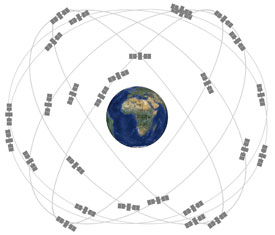
\includegraphics[width=0.3\textwidth]{images/constellation.jpg}}
\date{04. Dezember 2018}

\begin{document}
    \maketitle
    \begin{frame}{Inhalte}
        \tableofcontents
    \end{frame}
    \section{Grundlagen}
\begin{frame}{Grundlagen}
    \begin{block}{Betreiber}
        US-Regierung, Verteidigungsministerium
    \end{block}
    \begin{block}{Budget}
        2017: \$908,262 mil.\\
        2018: \$1,1 mrd
    \end{block}
    Bezahlt aus den Steuern der US-Bürger {\small [gps.gov]}
\end{frame}

\begin{frame}{Team Blackjack}
    \begin{columns}
        \begin{column}{0.5\textwidth}
            \begin{figure}
                \centering
                
\includegraphics[width=0.6\textwidth]{images/2sops.PNG}
            \end{figure}
            U.S. Air Force's\\
            2nd Space Operations Squadron
        \end{column}
        \begin{column}{0.5\textwidth}
            \begin{figure}
                \centering
                
\includegraphics[width=0.6\textwidth]{images/19sops.JPG}
            \end{figure}
            U.S. Air Force Reserve's\\
            19th Space Operations Squadron
        \end{column}
    \end{columns}
    ~\\~\\
    \centering{\small [gps.gov]}
\end{frame}

\begin{frame}{Historische Meilensteine}
    \begin{columns}
        \begin{column}{0.5\textwidth}
            \begin{itemize}
                \item[1957:] Sputnik
                \item[1964:] US-Marine, TRANSIT System
                \begin{itemize}
                    \item Bill Guier (Mathematiker)
                    \item George Weiffenbach (Physiker)
                \end{itemize}
                \item Kalter Krieg, Entwicklung verschiedener Systeme
                \item[1973:] Vereinigung zu NAVSTAR
                \item[1974:] Auftrag an Rockwell International
                \item[1986:] Start mit 18 Satelliten
                \item[1995:] 24 Satelliten
                \item[2010:] 30+ Satelliten im Betrieb
            \end{itemize}
        \end{column}
        \begin{column}{0.35\textwidth}
            \begin{figure}
                \centering
                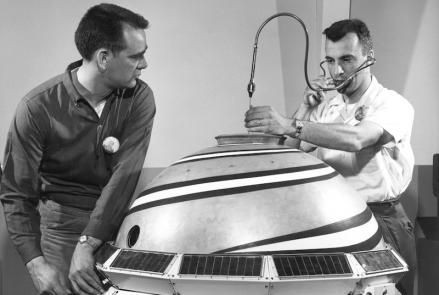
\includegraphics[width=0.35\paperwidth]{images/transit-satellite.jpg}
            \end{figure}
            Tests am zweiten Transit Satelliten, {\small [TimeAndNavigation]}
        \end{column}
    \end{columns}
\end{frame}

    \section{Aufbau}
\begin{frame}{Aufbau}
    \begin{itemize}
        \item Bodenstationen
        \item[]~
        \item Satelliten
    \end{itemize}
\end{frame}

\begin{frame}{Bodenstationen, {\small [gps.gov]}}
    \begin{figure}
        \centering
        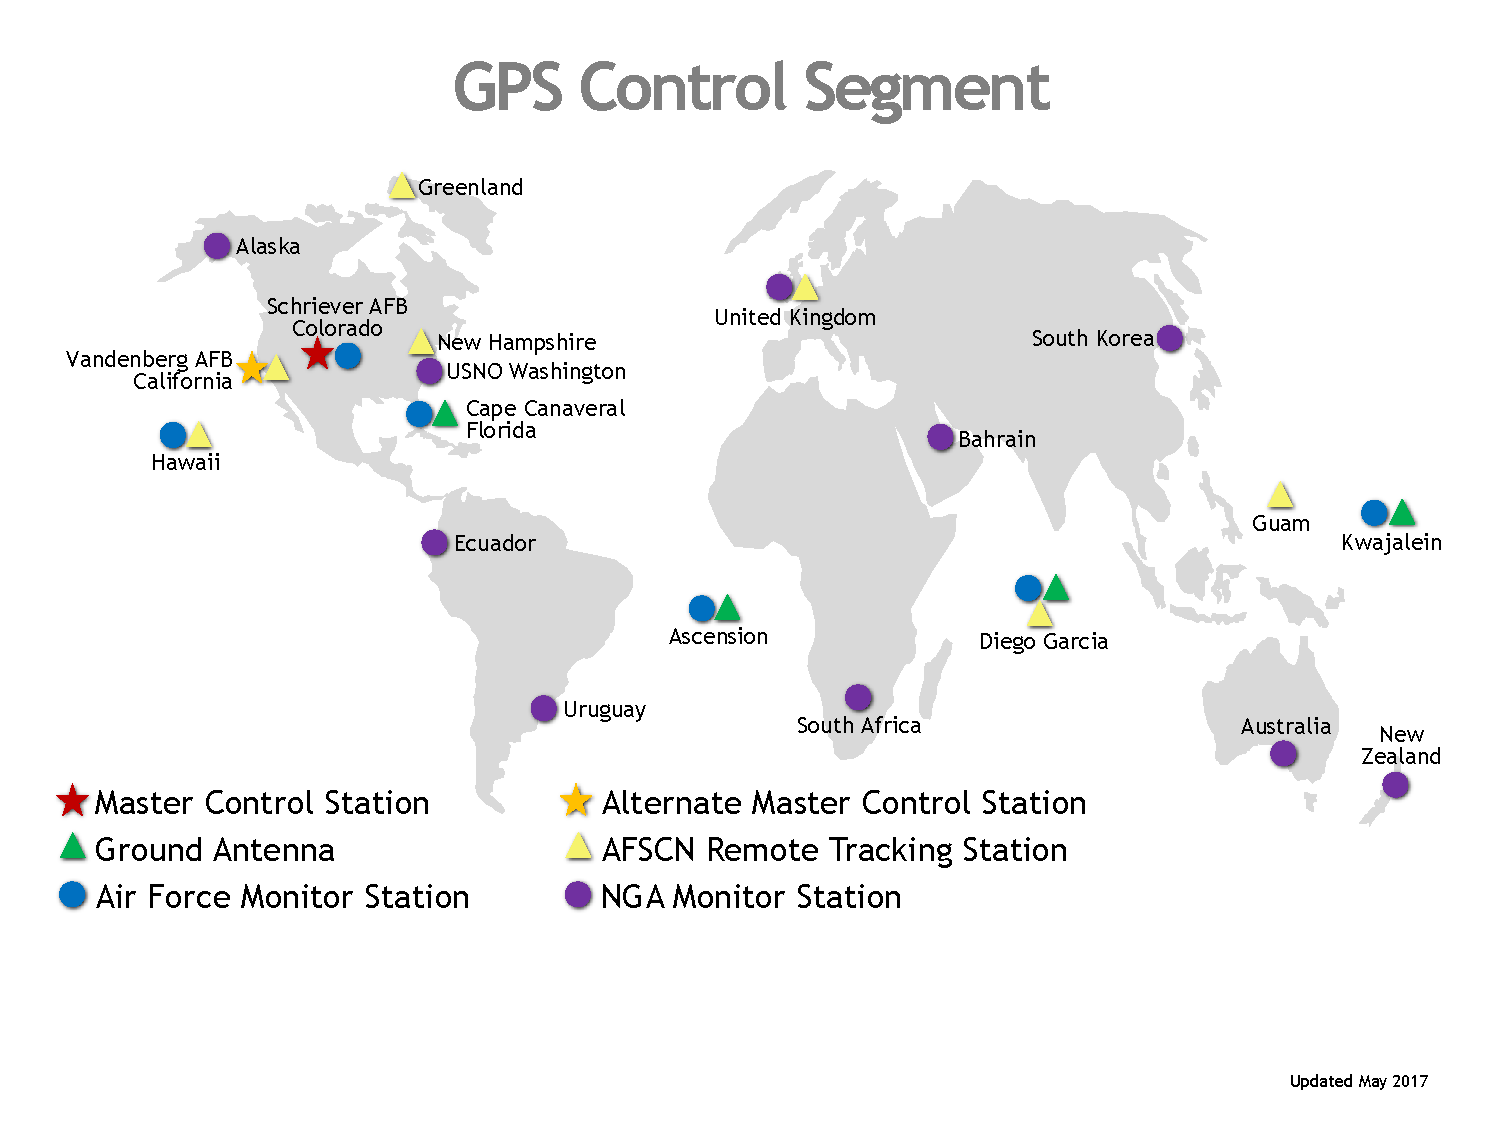
\includegraphics[width=\textwidth]{images/GPS-control-segment-map.pdf}
    \end{figure}
\end{frame}

\begin{frame}{Konstellation}
    \begin{columns}
        \begin{column}{0.5\textwidth}
            \begin{itemize}
                \item[Höhe:] \SI{20200}{\kilo\meter}
                \item[Umläufe:] 2 pro Tag
                \item[Orbitale:] 6, mit je 4 Satelliten
                \item[→] 4 Satelliten an jedem Ort sichtbar
                \item[2011:] Umpositionierung auf \textit{Expanable 24}\\mit 27 aktiven Satelliten
            \end{itemize}
        \end{column}
        \begin{column}{0.3\textwidth}
            \begin{figure}
                \centering
                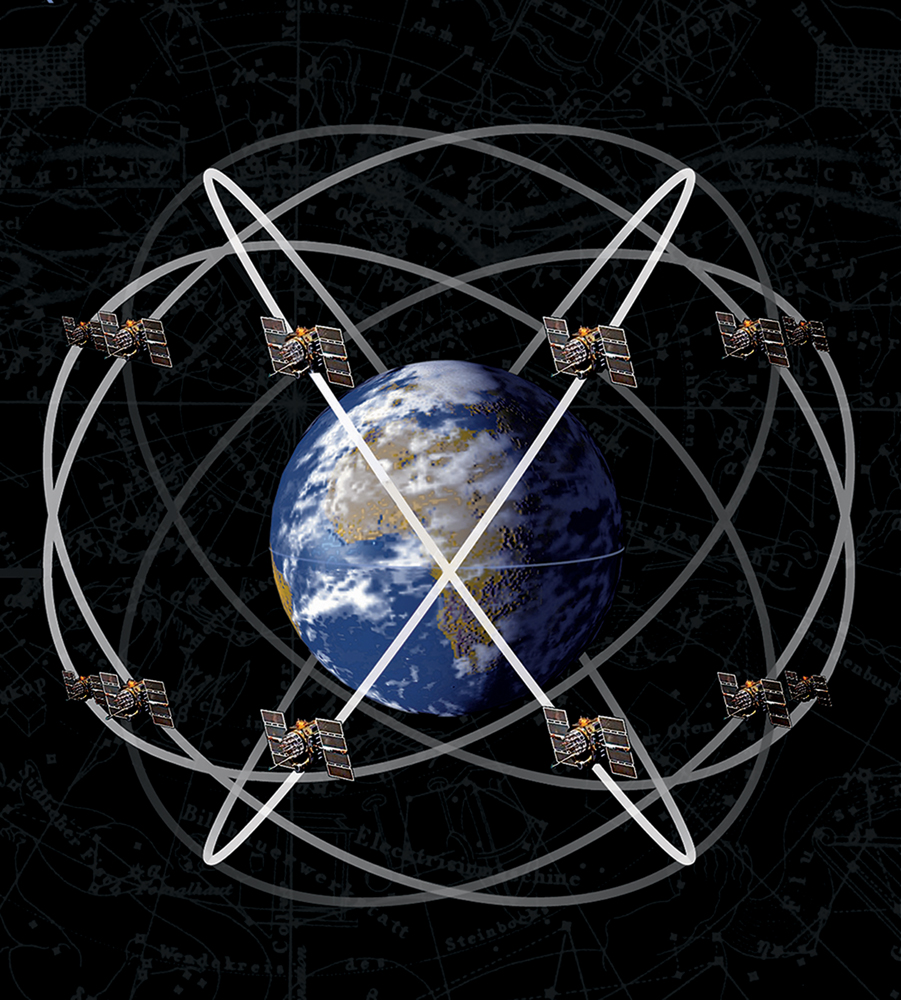
\includegraphics[width=\textwidth]{images/satelliten_schaubild.jpg}
            \end{figure}
            {\small [TimeAndNavigation]}
        \end{column}
    \end{columns}
\end{frame}

\begin{frame}{Die verschiedenen Satelliten im Überblick.}
    \begin{table}
        \begin{tabular}{c S[table-format=2.0] c S[table-format=2.1] c}
            \toprule
            {} & {Aktiv} & {Start} & {\enquote{MHD}} & {Änderungen} \\
            \midrule
            IIA   &  1 & 1990-1997 & 7.5 & \\
            IIR   & 11 & 1997-2004 & 7.5 & Onboard Uhrüberwachung \\
            IIR-M &  7 & 2005-2009 & 7.5 & Mehr und stärkere M(ilitär)signale \\
            IIF   & 12 & 2010-2016 & 12  & neue Uhr, bessere Signalabstrahlung \\
            III   &  0 & Dez 2018  & 15  & bessere Zuverlässigkeit, kein SA mehr \\
            IIIF  &  0 & Dez 2018  & 15  & $^{\---}"^{\---}$ , SAR kompatibel \\
            \bottomrule
        \end{tabular}
    \end{table}
\end{frame}

\begin{frame}{SA = selective Availability}
    ziviles GPS stören\\
    Grund: \textit{national security reasons}\\
    Abschaltung: 02.05.2000, 4 Uhr
    \begin{figure}
        \centering
        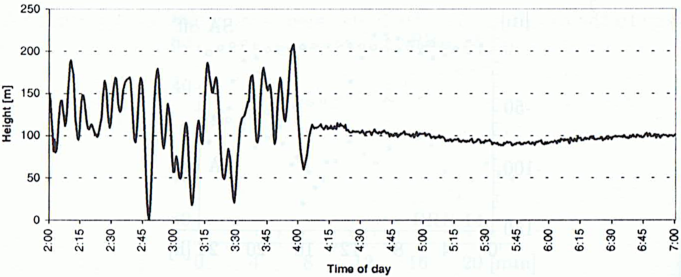
\includegraphics[width=\textwidth]{images/sa-hoehe.PDF}
    \end{figure}
    Höhenmessung in Kootwijk (Niederlande), 02.05.2000\;\;{\small [C,H-W,L](S.90)}
\end{frame}

\begin{frame}{GPS-Satelliten}
    \begin{columns}
        \begin{column}{0.5\textwidth}
            \begin{figure}
                \centering
                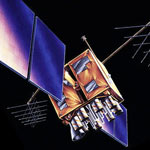
\includegraphics[height=0.6\textheight]{images/IIR.jpg}
            \end{figure}
            \centering{Typ IIR}
        \end{column}
        \begin{column}{0.5\textwidth}
            \begin{figure}
                \centering
                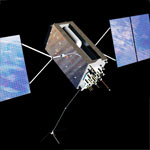
\includegraphics[height=0.6\textheight]{images/IIIA.jpg}
            \end{figure}
            \centering{Typ III}
        \end{column}
    \end{columns}
    \centering{\small [gps.gov]}
\end{frame}

\begin{frame}{NIST-7 Atomuhr}
    \begin{figure}
        \centering
        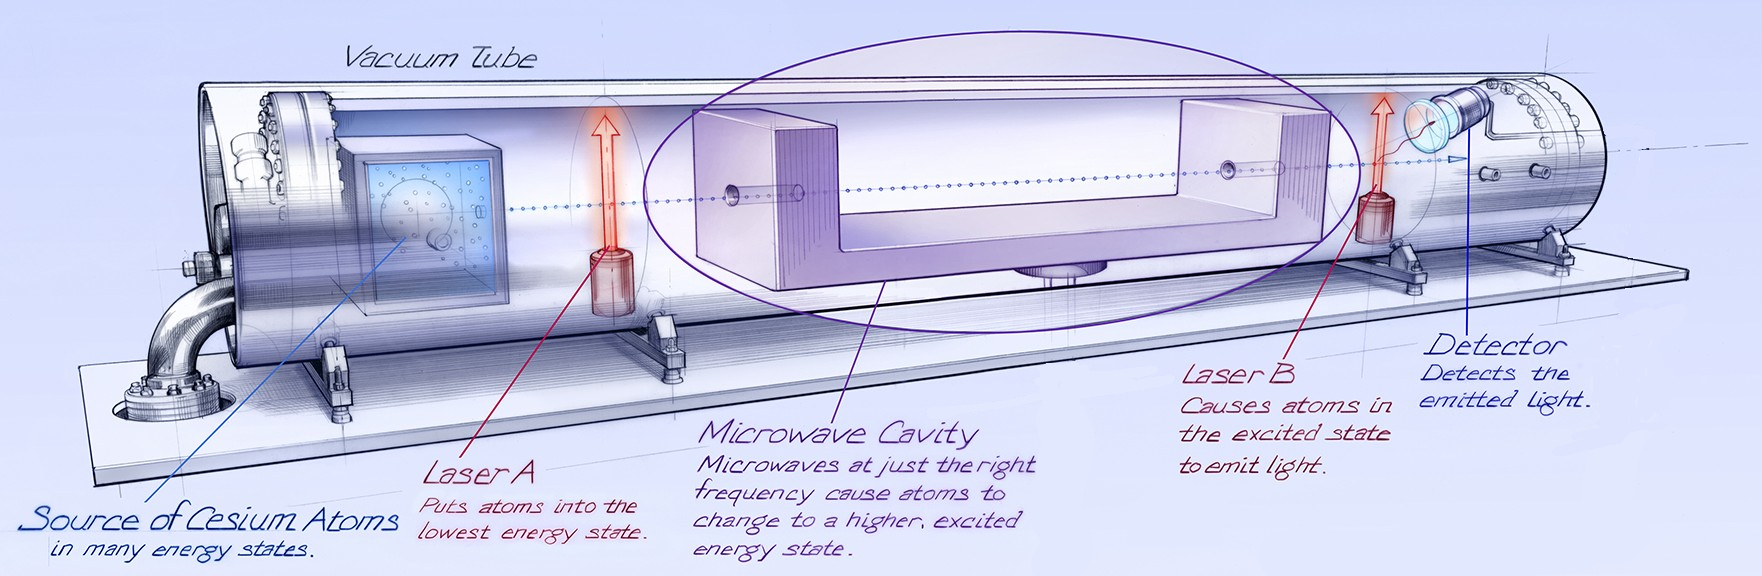
\includegraphics[width=\textwidth]{images/nist-7.jpg}
    \end{figure}
    \begin{columns}
        \begin{column}{0.5\textwidth}
            \begin{figure}
                \centering
                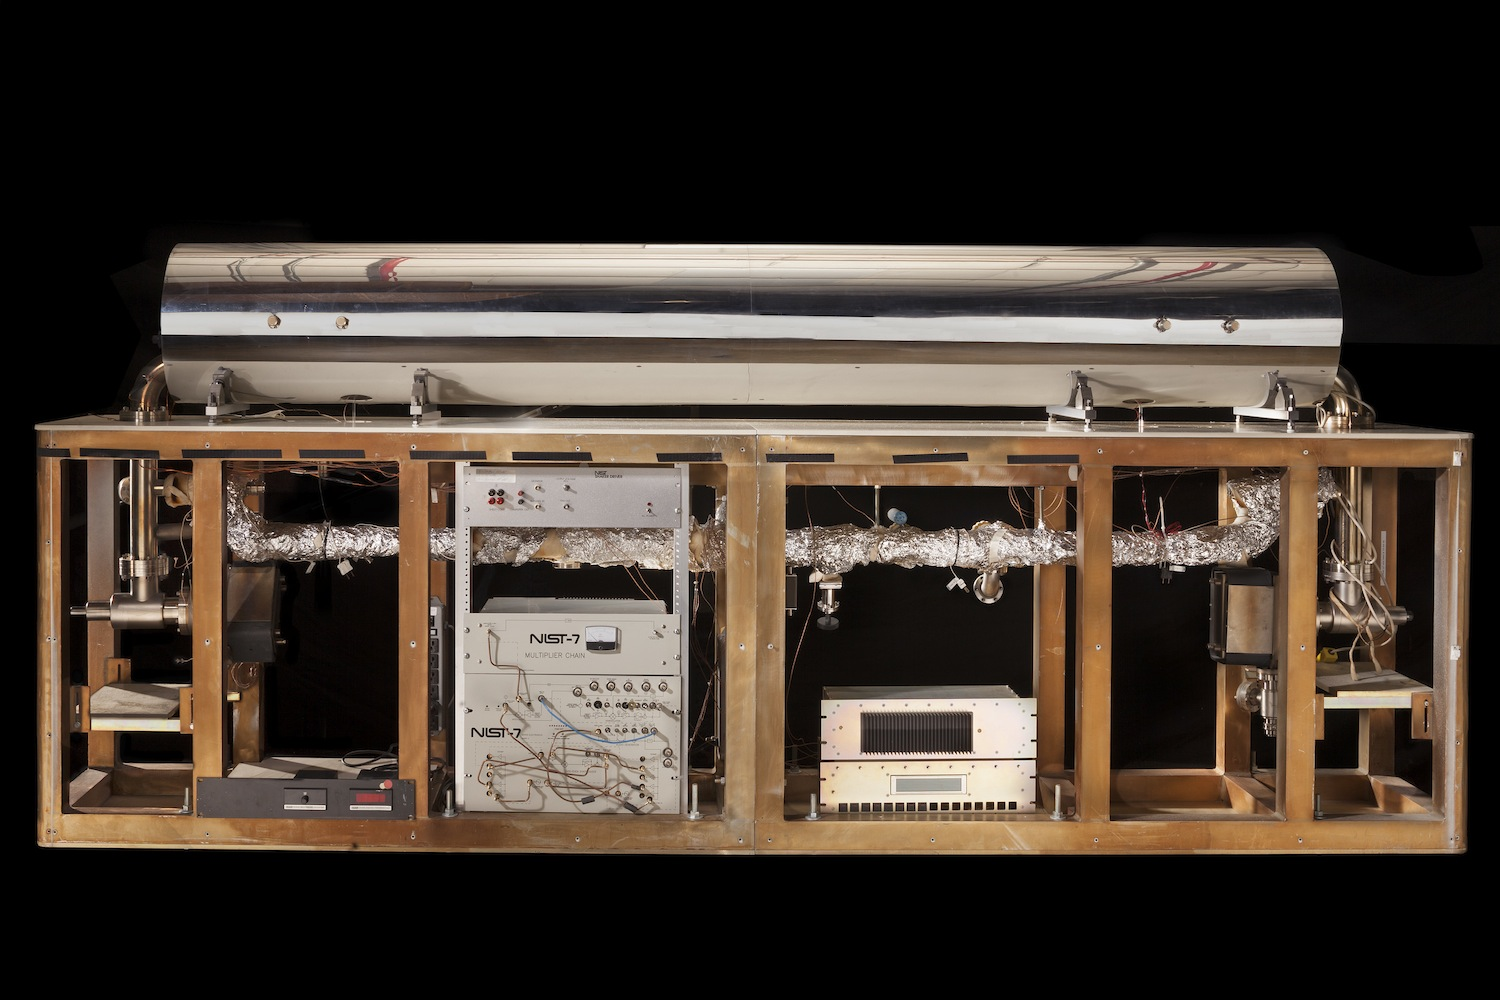
\includegraphics[height=0.4\textheight]{images/nist-7-real.jpg}
            \end{figure}
        \end{column}
        \begin{column}{0.5\textwidth}
            Ähnliche Methode zur Bestimmung\\
            von $\SI{1}{\second}$ als SI-Grundheiten\\
            {\small [TimeAndNavigation]}
        \end{column}
    \end{columns}
\end{frame}

    \section{Signale}
\label{sec:signale}

\begin{frame}{Frequenzen}
    \begin{columns}
        \begin{column}{0.5\textwidth}
            \centering{Verteilung der Frequenzen}
            \begin{table}
                \centering
                \begin{tabular}{c S[table-format=1.0]}
                    \toprule
                    {Satellit} & {\# Frequenzen} \\
                    \midrule
                    Block IIA   & 1 \\
                    Block IIR   & 2 \\
                    Block IIR-M & 3 \\
                    Block IIF   & 4 \\
                    GPS III     & 5 \\
                    GPS IIIF    & 5 \\
                    \bottomrule
                \end{tabular}
            \end{table}
        \end{column}
        \begin{column}{0.5\textwidth}
            \centering{Frequenzen der Frequenzen}
            \begin{table}
                \centering
                \begin{tabular}{c S[table-format=4.2]}
                    \toprule
                    {Name} & {$f\:/\:\si{\mega\hertz}$} \\
                    \midrule
                    L1 C/A  & $\num{1575.42}$ \\
                    L1 P(Y) & $\num{1575.42}$ \\
                    L2C     & $\num{1227.60}$ \\
                    L5      & $\num{1176.45}$ \\
                    L1C     & $\num{1575.42}$ \\
                    \bottomrule
                \end{tabular}
            \end{table}
            Grundfrequenz: $f_0 = \SI{10.23}{\mega\hertz}$
        \end{column}
    \end{columns}
\end{frame}

\begin{frame}{Das Signal}
    \begin{columns}
        \begin{column}{0.5\textwidth}
            Informationen im Signal
            \begin{itemize}
                \item Satellitenposition
                \item Zeit
                \item Uhrzeitkorrekturen
                \item Systeminformationen
                \end{itemize}\pause
        \end{column}
        \begin{column}{0.5\textwidth}
            \begin{figure}
                \centering
                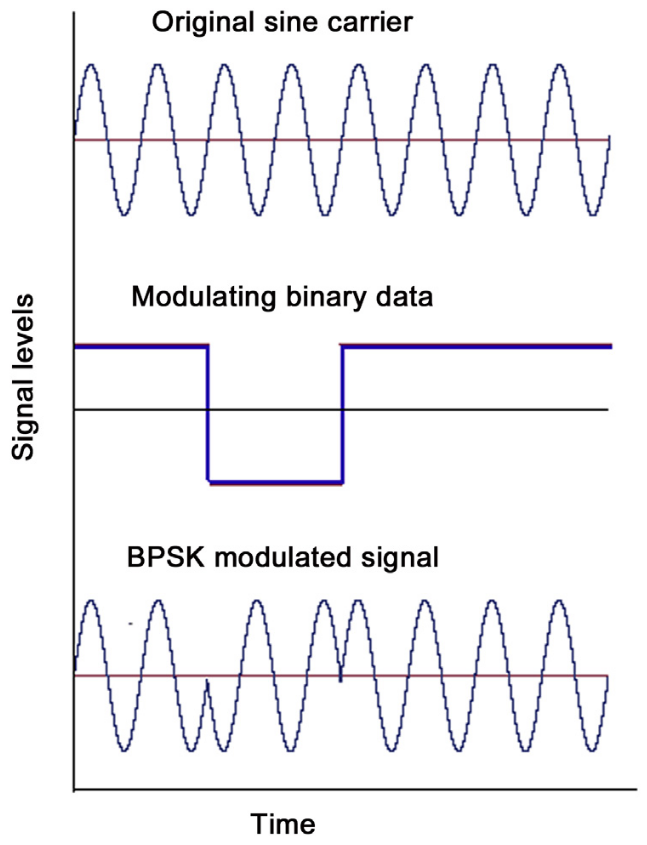
\includegraphics[width=0.6\textwidth]{images/signalzusammensetzung.png}
            \end{figure}
            Wellenzusammensetzung {\small[Acharya]}
        \end{column}
    \end{columns}
\end{frame}

    \section{Positionsbestimmung}

\begin{frame}{Phasenverschiebung}
    \begin{columns}
        \begin{column}{0.5\textwidth}
            \begin{align}
                φ^\text{S}(t) &= f\cdot t-\frac{ρ}{\symup{c}}f+f\cdotδ^\text{S} \\
                φ_\text{E}(t) &= f\cdot t+f\cdotδ^\text{E} \\
                φ^\text{S}_\text{E} &= -\frac{ρ}{\symup{c}}f-f\cdot\incrementδ \\
                &= \incrementφ^\text{S}_\text{E}|^t_{t_0}+N \\
                N &= \text{\# empfangene Signale}
            \end{align}
        \end{column}
        \begin{column}{0.5\textwidth}
            \begin{figure}
                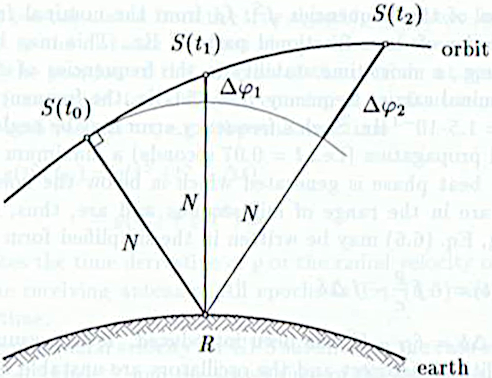
\includegraphics[width=\textwidth]{images/phasenverschiebung.jpg}
            \end{figure}
            \centering{\small[C,H-W,L]}
        \end{column}
    \end{columns}
\end{frame}

\begin{frame}{Zeitverzögerungen am Signal}
    S = Satellit, E = Empfänger
    \begin{align}
        t &= \text{Sende- /Empfangszeit} \\
        δ &= \text{zeitliche Verzögerungen, z.B. durch Rechenzeiten} \\
        t &= t(\text{GPS}) + δ
        \shortintertext{Zeitunterschied:}
        \increment t &= t_\text{E} - t^\text{S} = \increment t(\text{GPS}) +\incrementδ
        \shortintertext{Pseudoentfernung:}
        R &= \symup{c}\increment t = ρ + \symup{c}\incrementδ
        \shortintertext{Taylorreihe:}
        ρ\left(t_\text{E},\;t^\text{S}\right) &= ρ\left(t_\text{E},\;t^\text{S}+\increment t\right) = ρ\left(t^\text{S}\right)+\dot{ρ}\left(t^\text{S}\right)\cdot\increment t
        \shortintertext{Größe der ersten Korrektur:}
        \dot{ρ}\left(t^\text{S}\right)\cdot\increment t &\approx \SI{0.9}{\kilo\meter\per\second}\cdot\SI{0.07}{\second} =\SI{63}{\meter}
    \end{align}
\end{frame}

\begin{frame}{Ortskoordinaten}

\end{frame}

    \section{Literatur}
    \begin{frame}{Literatur}
        \nocite{*}
        \printbibliography
    \end{frame}
\end{document}
